\chapter[Inteligencia del Cliente al Tema Deserción]{Inteligencia del Cliente al Tema Deserción}
\label{ch:des}


Un aspecto importante del concepto de Inteligencia del Cliente, es entender las necesidades del consumidor. En el caso de este trabajo, se manejan los conceptos de IC aplicado a alumnos, para entender sus necesidades y motivaciones en terminar una carrera universitaria.\\

El siguiente desarrollo busca como objetivo ver las motivaciones de los alumnos, para convertirlos en constructos junto a sus asociaciones, los cuales entregarán métricas y variables para analizar el tema deserción. Las métricas y variables definidas en esta sección, ayudará a la selección de datos y construcción de los modelos, para luego aplicar las técnicas de minería de datos con la herramienta \textit{RapidMiner} a la base de datos de la entidad  privada.

\section{Entrevistas con Metodología de Metáforas}


Para captar las necesidades de los alumnos se utilizo la metodología de metáforas, en donde se le pide al entrevistado que recorte de 6 a 8 imágenes de revistas que representen para él, el concepto a evaluar. El concepto a evaluar en este caso, se representa con la pregunta principal ¿Qué te motiva a terminar la carrera?. (Ver Anexo A).\\

El marco muestral se define a partir de un segmento de cliente, para el caso de esta investigación, el segmento abarca a alumnos de educación superior de instituciones universitarias.\\

Como el objetivo de las entrevistas es encontrar las necesidades y motivaciones de los alumnos, se utilizará un muestreo no probabilístico, del tipo intencional o por conveniencia, que consiste en seleccionar individuos que son más fáciles de entrevistar \cite{muestra}.\\

El resultado de las entrevistas, permitirá generar constructos a partir de sus necesidades y motivaciones.\\



\subsection{Constructos}

Los constructos son definiciones interpretadas a partir de las asociaciones de las imágenes escogidas por los entrevistados, estas definiciones derivan en variables a contemplar para armar un modelo.\\ 

Los constructos recogidos en esta investigación reflejan el sentir del alumno en la carrera, los cuales se pueden plasmar en su formación como profesional y en sus sueños futuros.\\

\begin{figure}[H]
		\centering 
		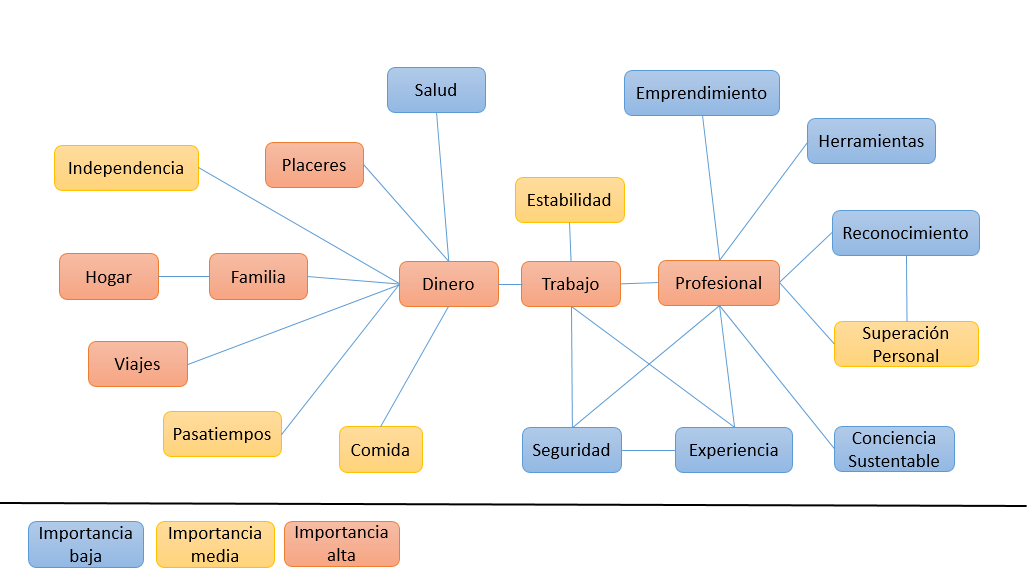
\includegraphics[width=12cm,height=7cm] {constructos.png} 
		\caption[Mapa de Consenso Generado]{Mapa de Consenso Generado}
		\label{fig:constru}
\end{figure}  

La Figura \ref{fig:constru} representa el \textit{Mapa de Consenso} generado a partir de los constructos obtenidos de las entrevistas, los más importantes son los que se repitieron en la mayoría de las entrevistas y son los principales insight de los alumnos al responder la pregunta ¿Qué te motiva a terminar la carrera?.\\

A continuación se detallan los constructos obtenidos, en donde las asociaciones son realizadas por los entrevistados, las definiciones son interpretaciones a las asociaciones, y las variables son los posibles datos ligados a las definiciones.\\    

\underline {Constructo 1 - Familia} \\
Asociaciones:
\begin{enumerate}
	\item Representa el compartir con la familia una situación económica estable.
	\item Tener una familia y tener dinero para mantener a la familia.
	\item El terminar una carrera implica tener un buen trabajo y mucho dinero, con el cual se puede optar a mejores condiciones de vida.
	\item Poder dar una buena educación a los hijos.
	\item Poder formar mi familia alegre y saludable.	
\end{enumerate}

Definición:\\
Un alumno que valore la familia, también valorará el tiempo que tiene para dedicar a esta, mientras estudia.\\
Una alumno que vive en comunas apartadas tendrá menos tiempo con la familia, lo que redunda en buscar lugares más cercanos.\\
Por otro lado es importante clasificar las carreras que otorgan un mayor bienestar para la familia.\\
Sumado a lo anterior de igual forma se debe analiza el impacto que tiene el deseo de estudiar la carrera.\\

Variables:
\begin{itemize}
	\item Distancia a universidad (comuna).
	\item Estudiar 3 primeras prioridades.
	\item Tiempo medio de encontrar trabajo estudiante egresado.
\end{itemize}


\underline {Constructo 2 - Independencia}\\ 
Asociaciones:
\begin{enumerate}
	\item Tener un espacio personal grande y vanguardista.
	\item Tener un auto para tener independencia.
	\item Tener la autonomía de vivir solo y tener un hogar
	\item Trabajar de forma independiente
	\item Poder vivir sola y tener mi departamento.	
\end{enumerate}

Definición:\\
Un alumno que valora la independencia, se encuentra más dispuesto a conseguir beneficios que lo ayuden económicamente, así como también trabajar durante la etapa estudiantil para satisfacer sus necesidades.\\

Variables:
\begin{itemize}
	\item Becas
	\item Créditos
	\item Beca alimenticia (Junaeb)
	\item Trabajador
\end{itemize}

\underline {Constructo 3 - Dinero}\\ 
Asociaciones:
\begin{enumerate}
	\item Representa el vehículo que podría adquirir teniendo recursos
	\item Felicidad y estabilidad amorosa, gracias a una buena situación económica.
	\item Poder acceder a muchas cosas, como bienes
	\item Poder comprar tecnología, gracias al buen sueldo que tendré
	\item Ser un profesional significa poder tener mucho dinero
\end{enumerate}

Definición:\\
Un alumno que tome en cuenta el dinero que ganará luego de egresar, debe tener conciencia en las estadísticas de su carrera, cual es la tasa de empleabilidad al 1er año de egreso y como aumentará su sueldo con los años de experiencia.\\

Variables:
\begin{itemize}
	\item Empleabilidad al 1er año
	\item Ingreso promedio al 4to año	
\end{itemize} 

\underline {Constructo 4 - Placeres}\\ 
Asociaciones:
\begin{enumerate}
	\item Tener un título, se asocia a disfrutar placeres de la vida.
	\item Representa las comodidades que uno podría tener una vez trabajando.	
	\item Poder obtener gustos exclusivos gracias al dinero.
	\item Comprar cosas exclusivas
\end{enumerate}

Definición:\\
Hace referencia a la libertad de poder gastar el dinero ganado en cosas o experiencias satisfactorias. Este constructro se encuentra asociado al constructo de Dinero, por lo que se aplican las mismas variables.\\

Variables:
\begin{itemize}
	\item Empleabilidad al 1er año
	\item Ingreso promedio al 4to año	
\end{itemize} 

\underline {Constructo 5 - Trabajo} \\
Asociaciones:
\begin{enumerate}
	\item Trabajar de forma relajada, ya que con el título tienes una base para dedicarse a lo que te gusta.
	\item Representa la adquisición de un bien raíz gracias al trabajo después de titulado
	\item Es lo que quiero llegar hacer, y tener un trabajo luego de titularme.	
	\item Poder relacionarse con otras personas y poder tener un trabajo sinergico
\end{enumerate}

Definición:\\
Representa a lo que se dedicará y obtendrá el alumno una vez titulado. Se relaciona al constructo Dinero y se asocian las mismas variables.\\

Variables:
\begin{itemize}
	\item Empleabilidad al 1er año
	\item Ingreso promedio al 4to año	
\end{itemize} 


\underline {Constructo 6 - Profesional} \\
Asociaciones:
\begin{enumerate}
	\item Generar aportes al trabajo, ser un buen profesional
	\item Tener un trabajo relacionado en redes informáticas y ser un buen profesional, para viajar por el mundo
	\item Encontrar un trabajo en una empresa prestigiosa.	
	\item Es a lo que uno aspira ser como ingeniero, teniendo buen puesto y reputación.
	\item Poder dedicarme al desarrollo de aplicaciones móviles.
\end{enumerate}

Definición:\\
Un alumno que valora el ser un profesional, tomará en cuenta el prestigio y excelencia de la institución, como también su formación profesional, por lo que será interesante saber si la institución se encuentra acreditada y si el alumno participa o ha participado en actividades que ayuden a validar sus capacidades.\\

Variables:
\begin{itemize}
	\item Acreditación Institucional
	\item Carrera Acreditada
	\item Talleres de Certificación
	\item Talleres de Desarrollo Profesional	
\end{itemize} 


\underline {Constructo 7 - Viajes} \\
Asociaciones:
\begin{enumerate}
	\item Tener la disponibilidad de tiempo y dinero, salir de la rutina, tener una vida más relajada
	\item Después de la carrera hay tiempo para disfrutar y conocer el mundo. 
	\item Libertad en poder ir a lugares diferentes y con mucha naturaleza
	\item Sin dinero no se puede viajar, y teniendo una carrera, uno puede ganar mucho dinero.	
	\item Poder viajar y hospedarse en buenos hoteles
\end{enumerate}

Definición:\\
Representa la libertad y la posibilidad de poder conocer nuevos lugares, sin preocupaciones de dinero.\\

Los viajes para los entrevistados representa el conocer otros países, si bien hace referencia a algo más vacacional, se puede asociar con las diferentes oportunidades que puede otorgar la institución para realizar intercambios, más puntual si el alumno a realizado un intercambio por medio de la institución.\\

Variables:
\begin{itemize}
	\item Alumno realizo intercambio
\end{itemize}


\underline {Constructo 8 - Pasatiempos} \\
Asociaciones:
\begin{enumerate}
	\item Tener una buena situación económica para disfrutar eventos culturales.
	\item Tener muchos libros por el gusto de leer.
	\item Poder tener la libertad de darse tiempos libres y hacer las cosas que uno quiere.
	\item Dedicar tiempo para mi persona y realizar lo que me gusta, la cocina.	
	\item Representa al parte artística que podría dedicarme teniendo recursos.
\end{enumerate}

Definición:\\
Hace referencia al tiempo disponible que tendrá, a poder cumplir y hacer lo que siempre le ha gustado hacer. Es importante para el alumno, que la institución a la cual pertenece disponga de talleres o facilidades que complementen sus estudios con los pasatiempos y si el alumno participa activamente de algún taller proporcionado por la institución.\\


Variables:
\begin{itemize}
	\item Taller deportivo o cultural 
	\item Beca deportiva
\end{itemize}


\underline {Constructo 9 - Hogar} \\
Asociaciones:
\begin{enumerate}
	\item Representa el compartir con la familia una situación económica estable.
	\item Tener una familia y tener dinero para mantener a la familia.
	\item Poder acceder a una buena casa en un buen barrio
	\item Tener una casa amplia y con bonita vista para recibir a la familia	
\end{enumerate}

Definición:\\
Representa independencia y unión familiar a través de la estabilidad económica. Se asocia a los constructos de Dinero y Familia\\

Variables:
\begin{itemize}
	\item Empleabilidad al 1er año
	\item Ingreso promedio al 4to año
	\item Distancia a universidad (comuna).
	\item Estudiar 3 primeras prioridades.
	\item Tiempo medio de encontrar trabajo estudiante egresado.	
\end{itemize} 

\underline {Constructo 10 - Comida} \\
Asociaciones:
\begin{enumerate}
	\item Tener una buena situación económica.
	\item Tener para comer y una vida sana.
	\item Representa los gustos que me podría dar, teniendo recursos.	
	\item Tener gustos sin depender económicamente de otras personas
	\item Tener un lugar agradable dentro de la casa
\end{enumerate}

Definición:\\

Hace mención a satisfacer la necesidad de alimento y darse una buena vida. Se asocia al constructo de Dinero junto a sus variables.\\

Variables:
\begin{itemize}
	\item Empleabilidad al 1er año
	\item Ingreso promedio al 4to año
	\item Beca alimenticia
\end{itemize} 

\underline {Constructo 11 - Experiencia} \\
Asociaciones:
\begin{enumerate}
	\item Estar listo para enfrentar el mundo laboral.
	\item Un profesional termina las cosas de manera más rápida, porque esta preparado.	
\end{enumerate}

Definición:\\

Hace referencia a sentirse preparado, a estar seguro en lo que se trabaja y poder cumplir de manera excelente. Es importante para el alumno ver la vinculación con el medio que tiene la institución y las prácticas ofrecidas.\\

Variables:
\begin{itemize}
	\item Prácticas realizadas
	\item Taller de Desarrollo Profesional	
\end{itemize} 

\underline {Constructo 12 - Superación personal} \\
Asociaciones:
\begin{enumerate}
	\item Cerrar una etapa de la vida, para pasar a una siguiente.
	\item Significa el cierre y el comienzo de una nueva etapa.
	\item Terminar una carrera transmite seguridad y sentirse útil para algo.
	\item Representa crecimiento personal y laboral	.
	\item Es el logro de cumplir con el objetivo de ser ingeniero.
\end{enumerate}

Definición:\\
Representa el alcanzar una meta, crecer, ser independiente y seguro. Esto se puede representar por los logros alcanzados por el alumno, como la cantidad de ramos aprobados en un semestre, promedio de notas o posición en ranking de alumno.\\

Variables:
\begin{itemize}
	\item Ramos aprobados por semestre
	\item Promedio de notas
	\item Ranking del alumno	
\end{itemize} 

\underline {Constructo 13 - Salud} \\
Asociaciones:
\begin{enumerate}
	\item Poder tener el dinero para obtener buenos tratamientos médicos		
\end{enumerate}

Definición:\\
Tener un titulo implica poder a acceder a una salud de calidad. Se asocia al constructo Dinero junto a sus variables.\\

Variables:
\begin{itemize}
	\item Empleabilidad al 1er año
	\item Ingreso promedio al 4to año	
\end{itemize} 


\underline {Constructo 14 - Seguridad} \\
Asociaciones:
\begin{enumerate}
	\item Desarrollar seguridad personal
	\item Tener una carrera te da seguridad de tener un buen trabajo	
	\item Salir de la carrera es un gran paso y te da libertar y seguridad en trabajar en lo que quieras
\end{enumerate}

Definición:\\
Hace referencia a que un titulo certifica las capacidades de una persona, haciéndolas sentir más seguras. Un alumno que busca seguridad laboral, buscara mejorar sus capacidades con certificaciones, es importante entonces que la institución a la que pertenece certifique los conocimientos del alumno.\\

Variables:
\begin{itemize}
	\item Talleres de certificación
	\item Acreditación institucional
	\item Carrera acreditada	
\end{itemize} 

\underline {Constructo 15 - Conciencia sustentable} \\
Asociaciones:
\begin{enumerate}
	\item Vida consciente con el planeta, a largo plazo
	\item Crear una fundación para ayudar a niños con discapacidad	
	\item Me gustaría tener un desarrollo sustentable, poder ayudar a la naturaleza con mi carrera
\end{enumerate}

Definición:\\
Se refiere a que una carrera entrega nociones y entendimiento sobre los efectos que tienen diferentes efectos sobre el planeta y la sociedad.\\  

Variables:
\begin{itemize}
	\item Participación en voluntariado social o ONG
	\item Ramos relacionado a conciencia sustentable	
\end{itemize} 

\underline {Constructo 16 - Reconocimiento} \\
Asociaciones:
\begin{enumerate}
	\item Representa el triunfo que puede llegar a tener como profesional.
	\item Terminar la carrera, da una sensación de libertad y triunfo. 
	\item Estar graduado y ser reconocido como un ingeniero.
	\item Como te observan las otras personas y como me proyecto como profesional	
	\item Refleja a mis padres, al terminar mi carrera ellos estarían orgullosos de mí
\end{enumerate}

Definición:\\
Representa a la sensación de un buen estatus, de crecimiento y aceptación. Se asocia al constructo Superación Personal junto a sus variables.\\

Variables:
\begin{itemize}
	\item Ramos aprobados por semestre
	\item Promedio de notas
	\item Ranking del alumno	
\end{itemize} 

\underline {Constructo 17 - Emprendimiento} \\
Asociaciones:
\begin{enumerate}
	\item Poder sacar un postgrado
	\item Poder dar clases en un futuro.
	\item Tener tiempo para poder realizar un curso de inglés y viajar al extranjero.
	\item Poder emprender con un negocio gourmet
	\item Tener mi propia oficina, trabajar con más gente y enseñar lo que sé	
\end{enumerate}

Definición:\\
Representa los sueños a futuros que se pueden cumplir gracias a un titulo. Para este constructo se relaciona la participación del alumno en distintas actividades que se relacione a emprendimiento, como talleres o concursos a través de la institución a la que pertenece.\\

Variables:
\begin{itemize}
	\item Talleres de emprendimiento	
\end{itemize} 

\underline {Constructo 18 - Estabilidad} \\
Asociaciones:
\begin{enumerate}
	\item Generar estabilidad y buenos lazos.
	\item Trabajar con personas, tener vida social 	
	\item Poder tener estabilidad económica y por ende tranquilidad
\end{enumerate}

Definición:\\
Representa que un titulo otorga poder estar seguro tanto económicamente como emocional. Un alumno con interés en tener una estabilidad económica como emocional, participara de actividades que lo ayuden a encontrar esa estabilidad, por ende las instituciones deben tener estas actividades, y el alumno participar de dichas actividades.\\

Variables:
\begin{itemize}
	\item Talleres Bienestar estudiantil
	\item Talleres de Desarrollo Profesional	
\end{itemize} 


\underline {Constructo 19 - Herramientas} \\
Asociaciones:
\begin{enumerate}
	\item Sueños de ser papá, de tener las herramientas para dar un buen pasar
	\item Los profesores motivan y te enseñan hacer trabajos de calidad	
	\item La universidad me da herramientas que me servirán para el futuro
	\item Representa las habilidades obtenidas en la carrera
\end{enumerate}

Definición:\\
Hace referencia al aprendizaje obtenido en la etapa universitaria. Es importante para el alumno tener las capacidades suficientes para poder ejercer sin problemas su titulo, por ende participara en actividades que le brinden estas herramientas.\\

Variables:
\begin{itemize}
	\item Talleres de certificación
	\item Talleres de Desarrollo Profesional	
\end{itemize} 

